%-----------------------------------------------------------------------------
%
%               Template for sigplanconf LaTeX Class
%
% Name:         sigplanconf-template.tex
%
% Purpose:      A template for sigplanconf.cls, which is a LaTeX 2e class
%               file for SIGPLAN conference proceedings.
%
% Guide:        Refer to "Author's Guide to the ACM SIGPLAN Class,"
%               sigplanconf-guide.pdf
%
% Author:       Paul C. Anagnostopoulos
%               Windfall Software
%               978 371-2316
%               paul@windfall.com
%
% Created:      15 February 2005
%
%-----------------------------------------------------------------------------


\documentclass[preprint]{sigplanconf}

% The following \documentclass options may be useful:

% preprint      Remove this option only once the paper is in final form.
% 10pt          To set in 10-point type instead of 9-point.
% 11pt          To set in 11-point type instead of 9-point.
% authoryear    To obtain author/year citation style instead of numeric.

\let\program\undefined % \program from acmtras2e conflicts with our program

\usepackage{amsmath}
\usepackage{graphicx}
\usepackage{epstopdf}
\usepackage{program}

%
% Load hyperref
%
\ifx\pdfoutput\undefined     %This is for regular output
  \def\nestedref{\protect\ref}
  \def\pdfbookmark#1#2{}%      % need this for non-pdf to work
\else %Use hyperref only if we run as pdflatex
  \usepackage[pdftex,
              colorlinks,
              linkcolor=blue,
              citecolor=red,
              pdfview=xyz,
              plainpages=false,
              pdfstartview=Fit,
              pdfhighlight=/P
              ]{hyperref}
  \def\nestedref{\protect\ref*}
      %Redefine the cross-referencing with no page references
 \long\def\genreftext#1#2#3#4{#1~#2}
\fi


% Magical incantation to allow \textbf{\texttt{}}
\DeclareFontShape{OT1}{cmtt}{bx}{n}
     {
      <5><6><7><8><9><10><10.95><12><14.4><17.28><20.74><24.88>cmttb10
      }{}


% hyphen-able fixed-width font
\newcommand{\ttt}[1]{{\texttt{\hyphenchar\font=`\-\relax #1}}}%`
\newcommand{\fixme}[1]{{\color{red} #1}}

\begin{document}

\special{papersize=8.5in,11in}
\setlength{\pdfpageheight}{\paperheight}
\setlength{\pdfpagewidth}{\paperwidth}

\conferenceinfo{Workshop on Programming Models for SIMD/Vector Processing '14}{February, 2014, Orlando, FL, USA}
\copyrightyear{2014}
\copyrightdata{978-1-nnnn-nnnn-n/yy/mm}
\doi{nnnnnnn.nnnnnnn}

% Uncomment one of the following two, if you are not going for the
% traditional copyright transfer agreement.

%\exclusivelicense                % ACM gets exclusive license to publish,
                                  % you retain copyright

%\permissiontopublish             % ACM gets nonexclusive license to publish
                                  % (paid open-access papers,
                                  % short abstracts)


\title{A SIMD Programming Model for Dart, JavaScript, and other dynamically typed scripting languages}

\authorinfo{John McCutchan}
           {Google Inc.}
           {johnmccutchan@google.com}
\authorinfo{Haitao Feng}
           {Intel Corp.}
           {haitao.feng@intel.com}
\authorinfo{Nicholas D. Matsakis}
           {Mozilla Research}
           {nmatsakis@mozilla.com}
\authorinfo{Zachary Anderson}
           {Google Inc.}
           {zra@google.com}
\authorinfo{Peter Jensen}
           {Intel Corp.}
           {peter.jensen@intel.com}

\maketitle

\begin{abstract}

It has not been possible to take advantage of the SIMD co-processors available
in all x86 and most ARM processors shipping today in dynamically typed scripting
languages. Web browsers have become a mainstream platform to deliver large and
complex applications with feature sets and performance comparable to native
applications, programmers must choose between Dart and JavaScript when writing
web programs. This paper introduces an explicit SIMD programming model for Dart
and JavaScript, we show that it can be compiled to efficient x86/SSE or ARM/Neon
code by both Dart and JavaScript virtual machines achieving a 300\%-600\% speed
increase across a variety of benchmarks. The result of this work is that more
sophisticated and performant applications can be built to run in web browsers.
The ideas introduced in this paper can also be used in other dynamically typed
scripting languages to provide a similarly performant interface to SIMD co-
processors.

\end{abstract}

\section{Introduction}

All x86 and many ARM processors shipping today include a dedicated single
instruction multiple data (SIMD) co-processor.  On x86 the SSE instruction set
allows for computing on 128-bit wide registers. ARM has the Neon instruction set
which allows for computing on 128-bit wide registers. Both SSE and Neon have
instructions for computing on 4 single precision floating point numbers
(\ttt{Float32x4}) and 4 signed integers (\ttt{Int32x4}) stored in 128-bit
registers. There are also instructions available for operating on 2 double
precision floating point numbers (\ttt{Float64x2}) as well as algorithm specific
instructions for operating on sound or pixel data.

Web browsers as a platform to deliver complex applications with feature sets and
performance that are comparable to native desktop applications have become
mainstream. All major browsers (Chrome, Firefox, Safari, and IE) include support
for displaying 3D graphics through WebGL, playing 3D positional audio through
WebAudio. These applications are written directly in JavaScript, Dart, or
compiled to JavaScript from C/C++ code through the LLVM based
Emscripten~\cite{emscripten} compiler. Starting in 2008 with the advent of the
V8 JavaScript virtual machine (VM) performance of JavaScript execution has
increased dramatically with browser vendors competing for the fastest JavaScript
VM. Dart is a new web programming language designed for performance with a
custom VM.

Despite the dramatic increase in performance it has not been possible for web
programs to access the dedicated SIMD co-processors. JavaScript is limited to
scalar operations on double precision floating point values and Dart is limited
to scalar operations on double precision floating point values and integers. In
this paper we introduce:

\begin{itemize}
\item
A SIMD programming model for Dart and JavaScript languages. The programming
model is high level but allows for explicit control over the SIMD co-processors.
It supports comparisons, branchless selection based on comparison results, and
efficient shuffling of scalar values within a SIMD value. The programming model
does not rely on compiler optimization passes like auto vectorization.

\item
Three (\ttt{Float32x4}, \ttt{Int32x4}, and \ttt{Float64x2}) new numeric value
types for Dart and JavaScript.

\item
Efficient array storage of the new numeric value types.

\item
How we generate performant machine code that is free of high level abstraction
in Dart and JavaScript VMs.

\item
An implementation of the programming model for the Dart VM that has shipped and
is used in production today.

\item
An implementation of the programming model for the V8 and SpiderMonkey
JavaScript VMs.

\item
Benchmarks that show (depending on the algorithm) a speedup of 300-600\% across
problem domains including real-time 3D graphics, numerical computation, ray
tracing, and cryptography.
\end{itemize}

\section{Lack of SIMD programmability for web applications}

Many algorithms can be sped up by taking advantage of SIMD co-processors. A
simple example is the averaging of an array of numbers. The top of
Figure~\ref{fig:average} shows a scalar implementation written in Dart. The
algorithm simply accumulates all the data points and computes the average by
dividing by the number of data points. The bottom of the figure shows a SIMD
implementation also written in Dart. This algorithm can trivially take advantage
of SIMD co-processors by adding 4 numbers at the same time.

\begin{figure}
\begin{small}
\begin{program}[style=tt, number=true]
do\tab{}uble scalar\_average(Float32List data) \{
  var sum = 0.0;
  fo\tab{}r (var i = 0; i < data.length; i++) \{
    sum += data[i];\untab{}
  \}
  return sum / data.length;\untab{}
\}
\end{program}
\end{small}
\ \ \\ \ \ \\
\begin{small}
\begin{program}[style=tt, number=true]
do\tab{}uble simd\_average(Float32x4List data) \{
  var sum = new Float32x4.zero();
  fo\tab{}r (var i = 0; i < data.length; i++) \{
    sum += data[i];\untab{}
  \}
  var total = sum.x + sum.y + sum.z + sum.w;
  return total / (data.length * 4);\untab{}
\}
\end{program}
\end{small}
\caption{Scalar (top) and SIMD (bottom) implementations of an algorithm to find
the average of an array of numbers.}
\label{fig:average}
\end{figure}

The bulk of the work is done in parallel and only after exiting the loop
does the program need to fall back to scalar computation when computing the
final sum and average.

If the \ttt{Float32x4} type were available to web programmers and the optimizing
compiler is successful in generating code that is free of memory allocation and
allows for temporary values to stay in CPU registers, the algorithm can be sped
up by 500\%. In the following section, we provide more details on the
programming model and how it can be efficiently compiled for x86 and ARM
processors.

\section{Bringing SIMD to the Web}

The SIMD programming model for Dart and JavaScript is designed to give direct
control to the programmer (or the Dart or C++ compiler generating JavaScript).
It introduces three new 128-bit wide value types: \ttt{Float32x4},
\ttt{Int32x4}, and \ttt{Float64x2}. Each value type stores scalar values in
multiple ``lanes''. For example, \ttt{Float32x4} has four single precision
floating point numbers in lanes labelled: x, y, z, and w. Note that w is the
fourth lane and not the first. Each instance is immutable and all operations
result in a new instance.

\subsection{Primitive Operations}

This section will focus on the \ttt{Float32x4} type. The other types offer
similar operations but can be limited by a lack of actual instructions in SSE or
Neon. For example, there is no \ttt{Int32x4} divide instruction in either SSE or
Neon instruction sets. Emulation of missing instructions is discussed in future
work.

\ttt{Float32x4} supports standard arithmetic operations (+, -, *, /) as well as
approximate square root, reciprocal square root, and reciprocal. It also
supports absolute value, minimum, maximum, and clamp operations. All of these
operations are performed for each lane. For example, the minimum value of two
\ttt{Float32x4} is the \ttt{Float32x4} with the minimum value of each individual
lane.

\subsection{Type Conversion}

Value cast operations between \ttt{Float32x4} and \ttt{Int32x4} as well as
\ttt{Float32x4} and \ttt{Float64x2} are available. In the conversion between
\ttt{Float32x4} and \ttt{Float64x2} only the x and y lanes are used.

Bit-wise cast operations between \ttt{Float32x4}, \ttt{Int32x4}, and
\ttt{Float64x2} are available. These do not interpret the lane values but
provide a mechanism to directly convert the 128-bit value between all type
pairs.

\subsection{Comparison and Branchless Selection}

When comparing SIMD values the result is not a single boolean value but a
boolean value for each lane. Consider the example of computing the minimum value
of two values. Figure~\ref{fig:min} shows the scalar and SIMD algorithms written
in Dart:

\begin{figure}
\begin{small}
\begin{program}[style=tt, number=true]
nu\tab{}m scalar\_min(num a, num b) \{
  if\tab{} (a <= b) \{
    return a;\untab{}
  \}
  return b;\untab{}
\}
\end{program}
\end{small}
\ \ \\ \ \ \\
\begin{small}
\begin{program}[style=tt, number=true]
Fl\tab{}oat32x4 simd\_min(Float32x4 a, Float32x4 b) \{
  Int32x4 mask = a.lessThanOrEqual(b);
  return mask.select(a, b);\untab{}
\}
\end{program}
\end{small}
\caption{The scalar (top) and SIMD (bottom) minimum function.}
\label{fig:min}
\end{figure}

The comparison results in an \ttt{Int32x4} value with lanes containing
\ttt{0xFFFFFFFF} or \ttt{0x0} when the lane comparison is true or false
respectively. The resulting mask is used to pick which value's lane should be
used.

\subsection{Lane Access and Shuffling}

Direct access to each lane of a \ttt{Float32x4} can be had by accessing the x,
y, z, or w instance properties. An example of this is shown in the average
algorithm. Shuffling the order of lanes can also be done. Reversing the order of
the lanes, in Dart:

\begin{small}
\begin{program}[style=tt]
Fl\tab{}oat32x4 reverse(Float32x4 v) \{
  return v.shuffle(Float32x4.WZYX);\untab{}
\}
\end{program}
\end{small}

The shuffle method uses an integer mask to reorder the lane values in v. All 256
combinations are supported.

Because each instance is immutable it is not possible to change the value stored
in one of the lanes. Methods, for example, \ttt{withX} allow for constructing
new instances that are copies of an existing instance with an individual lane
value changed. For example, in Dart:

\begin{small}
\begin{program}[style=tt]
var x = new Float32x4(1.0, 2.0, 3.0, 4.0);
var y = x.withX(5.0);
\end{program}
\end{small}

\subsection{Memory I/O}

Up until this point we have only discussed individual values but in order to be
a generally useful programming model, compact and cache-friendly array storage
of each type is introduced. \ttt{Float32x4List}, \ttt{Int32x4List}, and
\ttt{Float64x2List} offer contiguous storage of \ttt{Float32x4}, \ttt{Int32x4},
and \ttt{Float64x2} values. Figure~\ref{fig:load-store} shows loading and
storing SIMD values in Dart.

\begin{figure}
\begin{small}
\begin{program}[style=tt, number=true]
vo\tab{}id copy(\tab{}Float32x4List destination,
          Float32x4List source,
          int n) \{\untab{}
  fo\tab{}r (var i = 0; i < n; i++) \{
    var x = source[i];   // Load.\label{line:load}
    destination[i] = x;  // Store.\untab{}
  \}\untab{}
\}
\end{program}
\end{small}
\caption{The \ttt{copy} function copies an array of SIMD values.}
\label{fig:load-store}
\end{figure}

Note that on the load on line~\ref{line:load} a new instance of \ttt{Float32x4}
is constructed. In Sections~\ref{boxing} and~\ref{inlining} we discuss how the
memory allocation and instance construction is avoided in optimized code.

\subsection{Mapping from high level to low level}

The programming model is high level with each operation requiring a method call
on a heap allocated object and results in a new heap allocated object holding
the resulting value. Each value is immutable and storage of temporary values
cannot be reused. The design of the programming model was done with care so that
when optimized code is generated, the overhead of the high level programming
model can be removed. Almost all method calls will be mapped directly to a
single CPU instruction. Some operations require slightly longer instruction
sequences but so would a hand written assembly programming performing the same
operation. Instances will be stored directly inside CPU registers avoiding the
cost of memory allocation and object creation. The following section covers how
this is accomplished.

\section{Dart VM implementation}

We will now discuss the implementation details of the programming model in the
Dart VM. Section~\ref{JS} discusses the implementation for JavaScript.

\subsection{Unoptimized Code}

When a function is first compiled by the Dart VM the generated code is
completely generic. Every method call is looked up in the receiving object's
class's function table. Every temporary value is allocated in the heap as a full
object under control of the GC.

\subsection{Type Collection}

Using techniques developed by H\"{o}lzle et al.~\cite{typefeedback} and other
researchers, the unoptimized code collects important type information that is
used later by the optimizing compiler. At each method call the unoptimized code
maintains a cache mapping from receiver class id to address of the
class's corresponding function, as shown in Figure~\ref{fig:typecache}.

\begin{figure}
\begin{center}
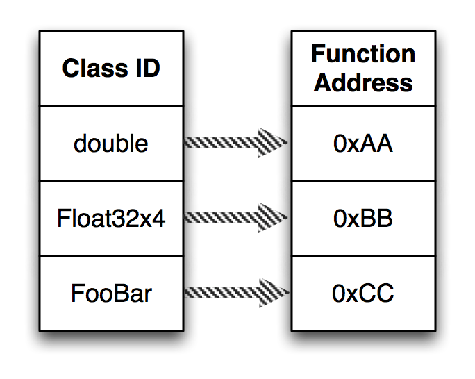
\includegraphics[width=0.25\textwidth]{figures/typecache.eps}
\end{center}
\caption{A call-site's type-cache.}
\label{fig:typecache}
\end{figure}

This data has two important uses:
\begin{itemize}
\item
Future execution of the unoptimized code will be faster if the receiving object
has a class id already seen at the call site. Execution is faster because
looking up the function for the method on the receiving object will result in a
cache hit, avoiding the expensive lookup and cache update.

\item
Types seen at a method call site are fed into the optimizing compiler and code
that optimistically expects to see the same type can be generated.
\end{itemize}

\subsection{Boxed and Unboxed Values}
\label{boxing}

The Dart compiler makes a distinction between boxed and unboxed~\cite{unboxing}
values. Boxed values are pointers to objects which are allocated in the heap
whose life cycle is managed by the GC. Unboxed values are stored in CPU
registers. Operations on unboxed values are much more efficient because the
values are already contained in CPU registers. Figure~\ref{fig:boxedobject}
shows the in-memory layout of an instance of \ttt{Float32x4}. The object header
contains information used for type collection and GC.

\begin{figure}
\begin{center}
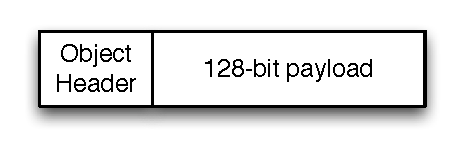
\includegraphics[width=0.25\textwidth]{figures/boxedobject.eps}
\end{center}
\caption{A boxed SIMD value.}
\label{fig:boxedobject}
\end{figure}

\subsection{Parameter Passing}

The Dart VM passes all method parameters and return value as boxed
instances. This can have a negative performance impact as unboxed values will be
boxed for the method call which will immediately unbox them again, as shown in
Figure~\ref{fig:boxunboxbox}.

\begin{figure}
\begin{center}
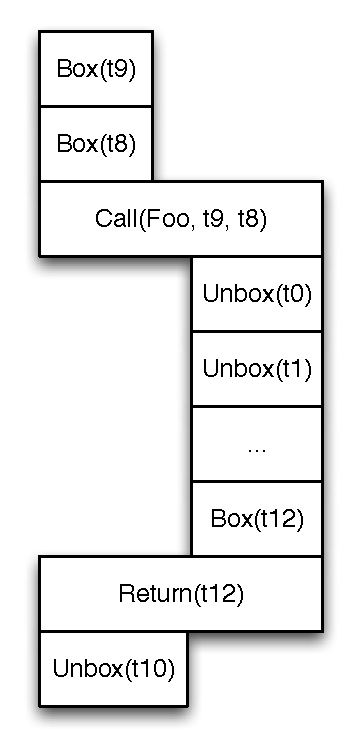
\includegraphics[width=0.25\textwidth]{figures/boxunboxbox.eps}
\end{center}
\caption{A SIMD value being boxed and unboxed for parameter passing and
function return.}
\label{fig:boxunboxbox}
\end{figure}

\subsection{Inlining}
\label{inlining}

Both the Dart VM and the JavaScript VMs make heavy use of inlining to avoid
method call invocation and unnecessary boxing of values. The first form of
inlining is similar to the inlining done in many compilers, the bodies of small
functions are copied into the calling function, replacing the method call. The
second form of inlining, replacement of runtime provided functions with compiler
intermediate representation (IR) instructions is the key to achieving high
performance with this programming model. Consider the code in
Figure~\ref{fig:unoptimized}.

\begin{figure}
\begin{small}
\begin{program}[style=tt, number=true]
Fl\tab{}oat32x4 compute(Float32x4 a, Float32x4 b) \{
  var c = a + b;
  var d = a * a;
  var e = b *  b;
  return c + d + e;\untab{}
\}
\end{program}
\end{small}
\ \ \\ \ \ \\
\begin{small}
\begin{program}[style=tt, number=true]
t0 $\leftarrow$ Call(+, a, b);
t1 $\leftarrow$ Call(*, a, a);
t2 $\leftarrow$ Call(*, b, b);
t3 $\leftarrow$ Call(+, t0, t1);
t4 $\leftarrow$ Call(+, t3, t2);
return t4;
\end{program}
\end{small}
\caption{A Dart function (top) and its compiled, but unoptimized code
(bottom). \ttt{Call} here indicates an expensive call into the Dart runtime.}
\label{fig:unoptimized}
\end{figure}

So long as the function \ttt{compute} has only ever been given \ttt{Float32x4}
instances, the compiler will recognize all of the call sites are monomorphic, in
other words, each call site has a single receiver class id and target function.
The type data collected in unoptimized code at each method call site is used to
determine whether this is the case or not. The function targets
\ttt{Float32x4\_Add} and \ttt{Float32x4\_Mul} are both provided by runtime and
the compiler knows how to replace them with IR instructions. As mentioned above,
the functions only accept and return boxed instances but the \ttt{Float32x4} IR
instructions only accept and return unboxed values.

\subsection{Optimized Code}

When inlining is successful the optimized code will be free of object
construction and method call invocations. Figure~\ref{fig:optimized} shows
the \ttt{compute} function from Figure~\ref{fig:unoptimized} after optimization.

\begin{figure}
\begin{small}
\begin{program}[style=tt, number=true]
if\tab{} (\!TypeMatch(a, Float32x4)) \{
  deoptimize();\untab{}
\}
if\tab{} (\!TypeMatch(b, Float32x4)) \{
  deoptimize();\untab{}
\}
t0 $\leftarrow$ unbox(a);
t1 $\leftarrow$ unbox(b);
t2 $\leftarrow$ BinaryFloat32x4Op+(t0, t1);
t3 $\leftarrow$ BinaryFloat32x4Op*(t0, t0);
t4 $\leftarrow$ BinaryFloat32x4Op*(t1, t1);
t5 $\leftarrow$ BinaryFloat32x4Op+(t2, t3);
t6 $\leftarrow$ BinaryFloat32x4Op+(t5, t4);
return box(t6);
\end{program}
\end{small}
\caption{The \ttt{compute} function after optimizing compilation. Here,
\ttt{BinaryFloat32x4Op\{+,*\}} indicate fast, inlined machine code routines.}
\label{fig:optimized}
\end{figure}

The optimized code first validates the class of each input value. If any of the
types do not match the expected type, the function is deoptimized. For more
details on deoptimization see Section~\ref{deoptimizing}. After being validated
the values are unboxed directly into CPU registers (tN) and the remaining
operations are performed directly in CPU registers with no memory I/O. The final
step is to box the result so it can be returned. Figure~\ref{fig:asm} shows the
final assembled result using Intel SSE SIMD instructions.

\begin{figure}[t]
\begin{small}
\begin{program}[style=tt]
\ \ \ \ \ \ \ \ \tab{}
        ;; CheckClass:14(v2)\untab{}
0x107822533 testb rdx,0x0x1
0x107822536 jz 0x107822607
0x10782253c movzxwq rbx,[rdx+0x1]
0x107822541 cmpl rbx,0x37
0x107822\tab{}544 jnz 0x107822607
        ;; CheckClass:14(v3)\untab{}
0x10782254a testb rcx,0x0x1
0x10782254d jz 0x107822612
0x107822553 movzxwq rbx,[rcx+0x1]
0x107822558 cmpl rbx,0x37
0x107822\tab{}55b jnz 0x107822612
        ;; v11 <- UnboxFloat32x4:14(v2)\untab{}
0x107822\tab{}561 \textbf{movups} xmm1, [rdx+0x7]
        ;; v14 <- UnboxFloat32x4:14(v3)\untab{}
0x107822\tab{}565 \textbf{movups} xmm2, [rcx+0x7]
        ;; ParallelMove xmm3 <- xmm1\untab{}
0x107822\tab{}569 \textbf{movaps} xmm3, xmm1
        ;; v4 <- BinaryFloat32x4Op:14(+, v11, v14)\untab{}
0x107822\tab{}56c \textbf{addps} xmm3, xmm2
        ;; ParallelMove xmm4 <- xmm1\untab{}
0x107822\tab{}56f \textbf{movaps} xmm4, xmm1
        ;; v5 <- BinaryFloat32x4Op:26(*, v11, v11)\untab{}
0x107822\tab{}572 \textbf{mulps} xmm4, xmm1
        ;; ParallelMove xmm1 <- xmm2\untab{}
0x107822\tab{}575 \textbf{movaps} xmm1, xmm2
        ;; v6 <- BinaryFloat32x4Op:38(*, v14, v14)\untab{}
0x107822\tab{}578 \textbf{mulps} xmm1, xmm2
        ;; v7 <- BinaryFloat32x4Op:50(+, v4, v5)\untab{}
0x107822\tab{}57b \textbf{addps} xmm3, xmm4
        ;; v8 <- BinaryFloat32x4Op:58(+, v7, v6)\untab{}
0x107822\tab{}57e \textbf{addps} xmm3, xmm1
        ;; v15 <- BoxFloat32x4:112(v8)\untab{}
0x107822581 movq r11,[r15+0x47]
0x107822588 movq rax,[r11]
0x10782258b addq rax,0x20
0x10782258f movq r11,[r15+0x4f]
0x107822596 cmpq rax,[r11]
0x107822599 jnc 0x1078225eb
0x10782259f  movq r11,[r15+0x47]
0x1078225a6 movq [r11],rax
0x1078225a9 subq rax,0x1f
0x1078225ad movq [rax-0x1],0x370200
0x1078225b5 movups [rax+0x7], xmm3
\end{program}
\end{small}
\caption{Optimized machine code generated by the Dart VM for the \ttt{compute}
function, SSE instructions bolded.}
\label{fig:asm}
\end{figure}

For readers unfamiliar with SSE, the following list describes the instructions
used in the example:

\begin{itemize}
\item \textbf{movups} Unaligned load or store of 128-bit value.
\item \textbf{movaps} Register move.
\item \textbf{addps} Add 4 single precision floating point numbers.
\item \textbf{mulps} Multiply 4 single precision floating point numbers.
\end{itemize}

\subsection{Register Allocation}

The Dart VM already supported unboxed double values which on x86 used the xmm
registers. The xmm registers are also needed for \ttt{Float32x4}, \ttt{Int32x4},
and \ttt{Float64x2} values. The register allocator was extended to support both
8 and 16 byte values stored in \ttt{xmmN} registers as well as allocate the
appropriate range of memory to spill values from registers to the stack when
register pressure requires spilling.

\subsection{Alignment}

SIMD instruction sets provide preferred memory I/O instructions that require the
memory address to be aligned on 16-byte boundaries. These instructions are
typically faster than the unaligned memory I/O instructions. All memory I/O
instructions emitted by the Dart VM are for unaligned addresses because the Dart
VM GC cannot guarantee object alignment.

\subsection{Deoptimization}
\label{deoptimizing}

After a function has been optimized if one of the values it uses violates the
optimistic type expectations, a deoptimization occurs resulting in the following
process:

\begin{itemize}
\item
Execution of optimized code stops.

\item
Optimized code is invalidated and disconnected from the function.

\item
Live unboxed values are boxed.

\item
Pointers to boxed values are stored in the correct locations of the unoptimized
codes stack frame.

\item
Execution of the function's unoptimized code begins at exactly the same point
that the deoptimization occurred.

\end{itemize}

An important thing to understand is that only functions which are provided
stable input types will be optimized.

\subsection{Port to ARM/Neon}

We have ported these SIMD operations in Dart to the Neon instruction set
provided by many ARM implementations.
%
In most cases the mapping from SSE instructions to Neon instructions is
straightforward.
%
In the case of the shuffle operation, the Neon instruction set lacks a fully
general single instruction.
%
In this, and a limited number of additional cases, we take advantage of the
overlap of the 128-bit ``Q'' registers with the 64-bit ``D'' and 32-bit ``F''
registers, and implement shuffles, etc., by simply manipulating the ``D'' and
``F'' registers that underly the ``Q'' registers.
%
Presently, these sequences are generated naively, and we are unaware of the
performance cost, though we assume it is small based on the benchmark results
in Section~\ref{sec:benchmarks}.
%
We leave as future work finding minimal Neon sequences to implement the more
general instructions provided by SSE.


\subsection{Implementation for JavaScript}
\label{JS}

The SIMD programming model for Dart is used for JavaScript as well. The 128-bit
wide value types are introduced, but as there are no class and operator
overloading language features in JavaScript, the syntax of the SIMD API is
different than Dart's. We introduced a SIMD global module with operations
grouped by type. The following example demonstrates the syntactic differences.
Figure~\ref{fig:jssimd} shows the translation of our \ttt{compute} function
into JavaScript.

\begin{figure}
\begin{small}
\begin{program}[style=tt, number=true]
fu\tab{}nction compute(a, b) \{
  var c = SIMD.float32x4.add(a, b);
  var d = SIMD.float32x4.mul(a, a);
  var e = SIMD.float32x4.mul(b, b);
  var t = SIMD.float32x4.add(c, d);
  return SIMD.float32x4.add(t, e);\untab{}
\}
\end{program}
\end{small}
\caption{Our \ttt{compute} function translated to JavaScript using our
experimental SIMD module.}
\label{fig:jssimd}
\end{figure}

\subsubsection{Implementation in V8}

The V8 implementation is conceptually similar to the implementation in the Dart
VM:

\begin{itemize}
\item
We added the 128-bit wide value constructor and SIMD API into full-codegen which
generates un-optimized code and optimized them in the Crankshaft which generates
optimized code.

\item
We allocated the 128-bit value in a heap object (with a header to indicate the
type) and garbage collect it when it is boxed; when the value is un-boxed, we
allocate it into a hardware 128-bit register (XMM register in the Intel IA32 and
X64 architectures).

\item
We inlined all the SIMD operations, inlining is the key technique for the
performance acceleration.

\item
Like the Dart VM, when transitioning from optimized to unoptimized code (due to
a deoptimization event) the unboxed values are boxed and pointers to the boxed
values are placed in the unoptimized codes stack frame.

\end{itemize}

Despite the many similarities, there are some important differences in the V8
implementation:

\begin{itemize}
\item
The unoptimized code does not collect type information for \ttt{Float32x4},
\ttt{Int32x4}, and \ttt{Float32x4} instances. Instead upon entry to a
SIMD.type.op function the types of the parameters are verified to match the
expected type. If they do not an exception is thrown.

\item
Because JavaScript is more dynamic than Dart and allows for object fields and
functions to be modified at runtime, for example, the \ttt{SIMD.float32x4.add}
method could have been overridden by the program. More checks are required to
ensure that these operations have not been replaced with user written code. When
this occurs inlining cannot be performed and performance suffers.

\end{itemize}

\subsubsection{Implementation in SpiderMonkey}

We are currently in the process of implementing the SIMD model for the
SpiderMonkey engine -- used in the Firefox web browser -- as well. At
the time of this writing, the SpiderMonkey implementation is able to
optimize several benchmarks, but it is not yet as mature as the V8 or
Dart implementations.

\begin{itemize}
\item
In the interpreter, 128-bit wide values are represented as objects,
each of which contains a pointer to a memory block storing the SIMD
value. This is not entirely faithful to the proposed specification, in
which the SIMD values are not objects but rather a new kind of
primitive JS value. Work on extending the set of primitive JS types
that SpiderMonkey supports is already underway, and we plan to
leverage that work once it completes so as to adhere more closely to
the specification.

\item
In JIT-optimized code, the SIMD values are aggressively unboxed. Calls
to SIMD operations are detected and replaced with native variants that
operate directly on the unboxed SIMD values. Extensions were needed to
the register allocator and bailout mechanism so that they could
support 128-bit values.

\item
If a bailout occurs, the unboxed SIMD values must be boxed into
objects so that the interpeter can resume execution. The same is true
whenever an unboxed value escapes out of the current function being
compiled, with the exception of stores into SIMD arrays.

\end{itemize}

\section{Benchmarks}
\label{sec:benchmarks}
In this section we introduce a variety of application domains that can benefit
from SIMD arithmetic. We discuss a variety of benchmarks that we have
implemented. Finally, we present benchmark results.

\subsection{Application Domains}
%
The ideas behind these benchmarks are twofold:
%
\begin{enumerate}
\item
They should reflect meaningful operations typically done with SIMD programming
\item
They should be small and easy to use for VM implementers to drive the
performance work in the VMs, when implementing JIT compiler support for those
operations
\end{enumerate}
%
For the benchmarks to be meaningful, they should cover at least some of the base
functionality required for application domains that benefit from SIMD
programming. Some (not all) of those domains are; 2D graphics
(e.g. filters, rendering) and 3D graphics (e.g. WebGL).  There are other
domains, such as computational fluid dynamics, finance (Black-Sholes),
cryptography, video processing, audio processing, etc. However, we haven't
extracted meaningful kernels for typical SIMD kernels from all of those domains
yet.
%
For the benchmarks to be small, they should mostly target select individual
operations.
%
The current set of benchmarks cover the following application domains:

\begin{itemize}
\item
\textbf{3D Graphics}
This application domain is tailor made for use of Float32x4 operations, because
most of the arithmetic involved operates on 4x4 or 3x3 matrices and vectors.
We've picked a few of the common operations to showcase the impact of SIMD.
%
The operations covered so far are:
\begin{itemize}
\item
\textbf{Vertex Transformation} Transformation of 4 element vector by 4x4 matrix
\item \textbf{Matrix Transpose} Transposition of 4x4 matrix
\item \textbf{Matrix Inversion} Compute the inverse of a 4x4 matrix
\item \textbf{Matrix Multiplication} Multiply two 4x4 matrices
\end{itemize}

\item \textbf{Cryptography}
This might not be a typical domain where use of SIMD operations can improve
performance, but we found a hot function in the implementation of the Rijndael
cipher
\footnote{\href{http://csrc.nist.gov/archive/aes/rijndael/Rijndael-ammended.pdf}
{Rijndael cipher}}. that would benefit, so we extracted it into a benchmark
kernel.

\begin{itemize}
\item \textbf{Shift Rows} (shift/rotate of row values in 4x4 matrix)
\end{itemize}

\item
\textbf{Vector Math Computations}
Math operations on small vectors, beyond simple algebraic operations (+,-,*,/),
typically include fairly complicated uses of SIMD operations, i.e. not just
individual SIMD instructions.  Intel provides a
Short Vector Math Library
\footnote{
\href{http://software.intel.com/sites/products/documentation/doclib/iss/2013/compiler/cpp-lin/index.htm\#GUID-7580634E-88D9-4B67-94ED-8472CCC5AF68.htm}
{Short Vector Math Library}} for that purpose for use in C/C++ SIMD code.
It is envisioned that such base math operations (sin, cos, exp, pow, etc) will
be useful for things like signal processing and physics engines.  In order to
show that a similar library could be implemented using the SIMD programming
API in Dart and JavaScript, with performance improvements equivalent to that of
highly optimized C/C++ functions, we have implemented a benchmark that computes
sine.

\begin{itemize}
\item \textbf{Sinex4} Compute 4 sine values at once.
\end{itemize}

\subsection{Results}

In this section we discuss  present benchmark results for four different benchmarks.
%
Full source code of these benchmarks is available from a GitHub
repository\footnote{\href{https://github.com/johnmccut
chan/ecmascript_simd/}{ECMAScript SIMD Polyfill}}.

\item
\textbf{Average} Averaging many floating point numbers.

\item
\textbf{Mandelbrot} Generating a Mandelbrot~\cite{mandelbrot} visualization.

\item
\textbf{MatrixMultiply} 4x4 matrix multiplication.

\item
\textbf{VectorTransform} 3D vertex transformation used for 3D rendering.
\end{itemize}


We ran these benchmarks on the Dart VM, V8, and SpiderMonkey using Dart and
JavaScript implementations as appropriate.
%
We used an Ubuntu 13.04 64-bit Linux system with an Intel CPU
(Intel(R) Xeon(R) CPU E5-2690 @ 2.90GHz).
%
We also ran the benchmarks on the Dart VM running on a Nexus 7, ARM Android
device.
%
Since ports to ARM/Neon are not yet complete for V8 and SpiderMonkey we did not
run the JavaScript implementations on the Nexus 7.


We ran each benchmark repeatedly until at least 2 seconds had elapsed, then
divided by the number of iterations in this time to arrive at the time taken
for a single iteration.
%
We report absolute times in microseconds for both the scalar and SIMD versions
of the benchmarks, as well as the SIMD speedup calculated as the scalar time
divided by the SIMD time.


\subsection{Discussion}

\begin{table}
\begin{center}
\begin{tabular}{|l|r|r|r|}
\hline
 Benchmark & Scalar   & SIMD     & Speedup \\
           & Time(us) & Time(us) &         \\
\hline
\hline
\multicolumn{4}{c}{Dart} \\
\hline
 Average & 381 & 36 & \textbf{10.5x} \\
\hline
 Mandelbrot & 330714 & 128750 & \textbf{2.6x} \\
\hline
 MatrixMultiply & 68 & 17 & \textbf{4.0x} \\
\hline
 VectorTransform & 25 & 5 & \textbf{5.0x} \\
\hline
\hline
\multicolumn{4}{c}{V8} \\
\hline
 Average & 208 & 35 & \textbf{5.9x} \\
 \hline
 Mandelbrot & 393167 & 109158 & \textbf{3.6x} \\
 \hline
 MatrixMultiply & 74 & 20 & \textbf{3.7x} \\
 \hline
 VectorTransform & 30 & 6 & \textbf{5.0x} \\
 \hline
\hline
\multicolumn{4}{c}{SpiderMonkey} \\
\hline
 Average & 116 & 21 & \textbf{5.5x} \\
 \hline
 Mandelbrot & 346333 & 152357 & \textbf{2.3x} \\
 \hline
 MatrixMultiply & 97 & 19 & \textbf{5.1x} \\
 \hline
 VectorTransform & 33 & 8 & \textbf{4.1x} \\
 \hline
\end{tabular}
\end{center}
\caption{Benchmark results for Dart, V8, and SpiderMonkey on our x64 Linux
machine.}
\label{tab:x64-benchmarks}
\end{table}


\begin{table}
\begin{center}
\begin{tabular}{|l|r|r|r|}
\hline
Benchmark & Scalar   & SIMD     & Speedup \\
          & Time(us) & Time(us) &         \\
\hline
\hline
Average & 1832 & 180 & \textbf{10.1x} \\
\hline
Mandelbrot & 1806000 & 892333 & \textbf{2.0x} \\
\hline
MatrixMultiply & 630 & 224 & \textbf{2.8x} \\
\hline
VectorTransform & 173 & 67 & \textbf{2.6x} \\
\hline
\end{tabular}
\end{center}
\caption{Benchmark results for Dart on our ARM Android device.}
\label{tab:arm-benchmarks}
\end{table}


The results of our benchmarks are shown in Tables~\ref{tab:x64-benchmarks}
and~\ref{tab:arm-benchmarks}.
%
Table~\ref{tab:x64-benchmarks} shows results on our Intel machine for Dart, V8,
and SpiderMonkey.
%
Table~\ref{tab:arm-benchmarks} shows results on a Nexus 7 device for Dart.
%
The benchmark data show significant speedups across a variety of algorithms,
implementations and across the two platforms when we use SIMD operations.
%
Further, our JavaScript and Dart benchmark kernels and timing harness are as
similar as possible, so it is possible not only to compare scalar and SIMD
implementations running on the same VM, but also to compare results across the
three VMs.


Thus, some of the results require some additional explanation.
%
The theoretical performance gain from SIMD should only be 4x, however a number
of our benchmarks show larger gains.
%
It is important to note that in the case of Dart and JavaScript that the scalar
code performs double precision arithmetic, while the SIMD code
performs single precision arithmetic.
%
The data in these scalar benchmarks is loaded from an array holding single
precision floating point values.
%
Thus, the scalar code must convert from single to double precision before
performing the calculation, while the SIMD code requires no conversion,
implying some saved time for the SIMD codes.


As for the Mandelbrot benchmark, Dart and SpiderMonkey achieved only speedups of
2.6x and 2.3x respectively, while V8 achieved a speedup of 3.6x.
%
The reason for the discrepancy is that the Dart VM has not fully implemented the
necessary inlining optimizations for the \ttt{Int32x4} type which is used in the
Mandelbrot benchmark.


\section{Related Work}

\subsection{C SSE Intrinsics}

C/C++ compilers offer SIMD intrinsic functions (\ttt{xmmintrin.h} and
\ttt{emmintrin.h}). At compile time these function calls are replaced with a
single instruction. Conceptually, the SIMD programming model for Dart and
JavaScript is similar but neither Dart nor JavaScript has static type
information available at compile time and instead, must rely on run-time type
collection (or enforcement) before the compiler can emit the SSE instructions.

\subsection{SIMD in C\#}

The Mono C\# compiler provided an API for SIMD~\cite{monosimd} programming. This
API is considered experimental and directly mimics the SSE instruction set
without any concern for portability across different SIMD instruction sets. The
SIMD programming model presented in this paper was designed to run across SSE
and Neon instruction sets and has been implemented for both.

\subsection{Auto-Vectorization}

Mozilla has experimented~\cite{mozillasimd} with an auto vectorization pass in
their JavaScript compiler. The focus of this work was on a gaussian blur
algorithm written in JavaScript. Speed gains of approximately 20\% were
achieved. This work was never merged and appears abandoned.

\section{Conclusions and Future Work}

In this paper we have presented a high level programming model that offers
direct control of SIMD co-processors to web programs in both Dart and
JavaScript. We have shown how both Dart and JavaScript VMs can avoid memory
allocation and the resulting garbage collector (GC) pressure by avoiding
instance creation with inlining and unboxed values. We have discussed the
implementations in both the Dart VM and V8. Finally, we have presented
benchmarks demonstrating the real world performance gains that this programming
model provides. Future work includes:

\begin{itemize}
\item
Support for wider (256-bit and 512-bit) SIMD register widths (AVX and AVX-512)
and the natural data types they offer, for example, \ttt{Float32x8} and
\ttt{Float32x16}. This includes generating correct code for wider register
widths on CPUs that only support 128-bit wide registers.

\item
Support for pixel processing by developing a portable abstraction around
instructions that are algorithm specific operating on 16 individual bytes.
Including support for saturating arithmetic operations.

\item
Support operations which do not have CPU instructions available, for example,
Int32x4 division.

\item
Supporting for passing and returning unboxed values directly, avoiding the
overhead of boxing values on method invocation and return.

\item
Support types that have few SIMD instructions, for example, \ttt{Int16x8}. Speed
ups may be seen on these types because efficient native code can that does N
scalar operations can be emitted directly.

\end{itemize}

\bibliographystyle{plain}
\bibliography{simdonweb}

\end{document}

%                       Revision History
%                       -------- -------
%  Date         Person  Ver.    Change
%  ----         ------  ----    ------

%  2013.06.29   TU      0.1--4  comments on permission/copyright notices

